\PassOptionsToPackage{unicode=true}{hyperref} % options for packages loaded elsewhere
\PassOptionsToPackage{hyphens}{url}
%
\documentclass[ignorenonframetext,aspectratio=43]{beamer}
\usepackage{pgfpages}
\setbeamertemplate{caption}[numbered]
\setbeamertemplate{caption label separator}{: }
\setbeamercolor{caption name}{fg=normal text.fg}
\beamertemplatenavigationsymbolsempty
% Prevent slide breaks in the middle of a paragraph:
\widowpenalties 1 10000
\raggedbottom
\setbeamertemplate{part page}{
\centering
\begin{beamercolorbox}[sep=16pt,center]{part title}
  \usebeamerfont{part title}\insertpart\par
\end{beamercolorbox}
}
\setbeamertemplate{section page}{
\centering
\begin{beamercolorbox}[sep=12pt,center]{part title}
  \usebeamerfont{section title}\insertsection\par
\end{beamercolorbox}
}
\setbeamertemplate{subsection page}{
\centering
\begin{beamercolorbox}[sep=8pt,center]{part title}
  \usebeamerfont{subsection title}\insertsubsection\par
\end{beamercolorbox}
}
\AtBeginPart{
  \frame{\partpage}
}
\AtBeginSection{
  \ifbibliography
  \else
    \frame{\sectionpage}
  \fi
}
\AtBeginSubsection{
  \frame{\subsectionpage}
}
\usepackage{lmodern}
\usepackage{amssymb,amsmath}
\usepackage{ifxetex,ifluatex}
\usepackage{fixltx2e} % provides \textsubscript
\ifnum 0\ifxetex 1\fi\ifluatex 1\fi=0 % if pdftex
  \usepackage[T1]{fontenc}
  \usepackage[utf8]{inputenc}
  \usepackage{textcomp} % provides euro and other symbols
\else % if luatex or xelatex
  \usepackage{unicode-math}
  \defaultfontfeatures{Ligatures=TeX,Scale=MatchLowercase}
\fi
\usecolortheme{beaver}
% use upquote if available, for straight quotes in verbatim environments
\IfFileExists{upquote.sty}{\usepackage{upquote}}{}
% use microtype if available
\IfFileExists{microtype.sty}{%
\usepackage[]{microtype}
\UseMicrotypeSet[protrusion]{basicmath} % disable protrusion for tt fonts
}{}
\IfFileExists{parskip.sty}{%
\usepackage{parskip}
}{% else
\setlength{\parindent}{0pt}
\setlength{\parskip}{6pt plus 2pt minus 1pt}
}
\usepackage{hyperref}
\hypersetup{
            pdftitle={Missing Data Imputation},
            pdfauthor={Stef van Buuren, University of Utrecht \& TNO},
            pdfborder={0 0 0},
            breaklinks=true}
\urlstyle{same}  % don't use monospace font for urls
\newif\ifbibliography
\usepackage{color}
\usepackage{fancyvrb}
\newcommand{\VerbBar}{|}
\newcommand{\VERB}{\Verb[commandchars=\\\{\}]}
\DefineVerbatimEnvironment{Highlighting}{Verbatim}{commandchars=\\\{\}}
% Add ',fontsize=\small' for more characters per line
\usepackage{framed}
\definecolor{shadecolor}{RGB}{248,248,248}
\newenvironment{Shaded}{\begin{snugshade}}{\end{snugshade}}
\newcommand{\AlertTok}[1]{\textcolor[rgb]{0.94,0.16,0.16}{#1}}
\newcommand{\AnnotationTok}[1]{\textcolor[rgb]{0.56,0.35,0.01}{\textbf{\textit{#1}}}}
\newcommand{\AttributeTok}[1]{\textcolor[rgb]{0.77,0.63,0.00}{#1}}
\newcommand{\BaseNTok}[1]{\textcolor[rgb]{0.00,0.00,0.81}{#1}}
\newcommand{\BuiltInTok}[1]{#1}
\newcommand{\CharTok}[1]{\textcolor[rgb]{0.31,0.60,0.02}{#1}}
\newcommand{\CommentTok}[1]{\textcolor[rgb]{0.56,0.35,0.01}{\textit{#1}}}
\newcommand{\CommentVarTok}[1]{\textcolor[rgb]{0.56,0.35,0.01}{\textbf{\textit{#1}}}}
\newcommand{\ConstantTok}[1]{\textcolor[rgb]{0.00,0.00,0.00}{#1}}
\newcommand{\ControlFlowTok}[1]{\textcolor[rgb]{0.13,0.29,0.53}{\textbf{#1}}}
\newcommand{\DataTypeTok}[1]{\textcolor[rgb]{0.13,0.29,0.53}{#1}}
\newcommand{\DecValTok}[1]{\textcolor[rgb]{0.00,0.00,0.81}{#1}}
\newcommand{\DocumentationTok}[1]{\textcolor[rgb]{0.56,0.35,0.01}{\textbf{\textit{#1}}}}
\newcommand{\ErrorTok}[1]{\textcolor[rgb]{0.64,0.00,0.00}{\textbf{#1}}}
\newcommand{\ExtensionTok}[1]{#1}
\newcommand{\FloatTok}[1]{\textcolor[rgb]{0.00,0.00,0.81}{#1}}
\newcommand{\FunctionTok}[1]{\textcolor[rgb]{0.00,0.00,0.00}{#1}}
\newcommand{\ImportTok}[1]{#1}
\newcommand{\InformationTok}[1]{\textcolor[rgb]{0.56,0.35,0.01}{\textbf{\textit{#1}}}}
\newcommand{\KeywordTok}[1]{\textcolor[rgb]{0.13,0.29,0.53}{\textbf{#1}}}
\newcommand{\NormalTok}[1]{#1}
\newcommand{\OperatorTok}[1]{\textcolor[rgb]{0.81,0.36,0.00}{\textbf{#1}}}
\newcommand{\OtherTok}[1]{\textcolor[rgb]{0.56,0.35,0.01}{#1}}
\newcommand{\PreprocessorTok}[1]{\textcolor[rgb]{0.56,0.35,0.01}{\textit{#1}}}
\newcommand{\RegionMarkerTok}[1]{#1}
\newcommand{\SpecialCharTok}[1]{\textcolor[rgb]{0.00,0.00,0.00}{#1}}
\newcommand{\SpecialStringTok}[1]{\textcolor[rgb]{0.31,0.60,0.02}{#1}}
\newcommand{\StringTok}[1]{\textcolor[rgb]{0.31,0.60,0.02}{#1}}
\newcommand{\VariableTok}[1]{\textcolor[rgb]{0.00,0.00,0.00}{#1}}
\newcommand{\VerbatimStringTok}[1]{\textcolor[rgb]{0.31,0.60,0.02}{#1}}
\newcommand{\WarningTok}[1]{\textcolor[rgb]{0.56,0.35,0.01}{\textbf{\textit{#1}}}}
\usepackage{longtable,booktabs}
\usepackage{caption}
% These lines are needed to make table captions work with longtable:
\makeatletter
\def\fnum@table{\tablename~\thetable}
\makeatother
\usepackage{graphicx,grffile}
\makeatletter
\def\maxwidth{\ifdim\Gin@nat@width>\linewidth\linewidth\else\Gin@nat@width\fi}
\def\maxheight{\ifdim\Gin@nat@height>\textheight\textheight\else\Gin@nat@height\fi}
\makeatother
% Scale images if necessary, so that they will not overflow the page
% margins by default, and it is still possible to overwrite the defaults
% using explicit options in \includegraphics[width, height, ...]{}
\setkeys{Gin}{width=\maxwidth,height=\maxheight,keepaspectratio}
\setlength{\emergencystretch}{3em}  % prevent overfull lines
\providecommand{\tightlist}{%
  \setlength{\itemsep}{0pt}\setlength{\parskip}{0pt}}
\setcounter{secnumdepth}{0}

% set default figure placement to htbp
\makeatletter
\def\fps@figure{htbp}
\makeatother


\title{Missing Data Imputation}
\providecommand{\subtitle}[1]{}
\subtitle{Overview of General Issues and Solutions}
\author{Stef van Buuren, University of Utrecht \& TNO}
\date{December 19, 2019; Building Multi-Source Databases for Comparative
Analyses}

\begin{document}
\frame{\titlepage}

\begin{frame}
\tableofcontents[hideallsubsections]
\end{frame}
\begin{frame}{Overview}
\protect\hypertarget{overview}{}

\begin{itemize}
\tightlist
\item
  Missing data and harmonization
\item
  Multiple imputation in a nutshell
\item
  Alternatives for recoding
\item
  Imputation of multilevel data
\end{itemize}

\end{frame}

\begin{frame}[fragile]{Why this course}
\protect\hypertarget{why-this-course}{}

\begin{itemize}
\tightlist
\item
  Missing data are everywhere
\item
  Harmonization is an attempt to solve a missing data problem
\item
  Ad-hoc fixes do not (always) work
\item
  Multiple imputation is broadly applicable, yield correct statistical
  inferences
\item
  Goal of the course: introduce \texttt{mice} as a way to think about
  data harmonization
\end{itemize}

\end{frame}

\begin{frame}{Course materials}
\protect\hypertarget{course-materials}{}

\begin{itemize}
\item
  URL to github site
\item
  Materials:
  \url{https://www.asc.ohio-state.edu/dataharmonization/wp-content/uploads/2019/12/Workshop-Missing-Data-Imputation-Materials-Kotnarowski-2019-FINAL.pdf}
\end{itemize}

\end{frame}

\begin{frame}[fragile]{Reading materials}
\protect\hypertarget{reading-materials}{}

\begin{itemize}
\tightlist
\item
  Van Buuren, S. and Groothuis-Oudshoorn, C.G.M. (2011). \texttt{mice}:
  Multivariate Imputation by Chained Equations in \texttt{R}. Journal of
  Statistical Software, 45(3), 1--67.
  \url{https://www.jstatsoft.org/article/view/v045i03}
\item
  Van Buuren, S. (2018). Flexible Imputation of Missing Data. Second
  Edition. Chapman \& Hall/CRC, Boca Raton, FL.
  \url{https://stefvanbuuren.name/fimd}
\end{itemize}

\end{frame}

\begin{frame}{}
\protect\hypertarget{section}{}

\centering{
\includegraphics[height=9cm,keepaspectratio=true]{figures/cover_border.png}}

\end{frame}

\begin{frame}{Today's schedule}
\protect\hypertarget{todays-schedule}{}

\begin{longtable}[]{@{}llll@{}}
\toprule
Slot & Time & What & Topic\tabularnewline
\midrule
\endhead
A & 10.00-11.30 & L & Multiple imputation intro\tabularnewline
~ & 11.30-11.45 & ~ & COFFEE/TEA\tabularnewline
B & 11.45-13:15 & L & Imputation for harmonisation\tabularnewline
~ & 13.15-14.30 & ~ & LUNCH\tabularnewline
C & 14.30-16.00 & P & Lab session: Kotnarowski, IFiS\tabularnewline
~ & 13.15-14.30 & ~ & COFFEE/TEA\tabularnewline
D & 16.15-17.30 & P & Lab session: Kotnarowski, IFiS\tabularnewline
\bottomrule
\end{longtable}

\end{frame}

\begin{frame}{Definition of missing values}
\protect\hypertarget{definition-of-missing-values}{}

\begin{itemize}
\tightlist
\item
  Missing values are those values that are not observed
\item
  Values do exist in theory, but we are unable to see them
\end{itemize}

\end{frame}

\begin{frame}{Some confusing terminology}
\protect\hypertarget{some-confusing-terminology}{}

\begin{itemize}
\tightlist
\item
  Complete data = Observed data + Unobserved data
\item
  Incomplete data = Observed data
\item
  Missing data = Unobserved data
\item
  Complete cases = Subset of rows without missing values
\item
  Complete variables = Subset of columns without missing values
\end{itemize}

\end{frame}

\begin{frame}{Complete data}
\protect\hypertarget{complete-data}{}

\begin{center}\includegraphics[height=3in]{Lecture_1_files/figure-beamer/unnamed-chunk-3-1} \end{center}

\end{frame}

\begin{frame}{Incomplete data = observed data}
\protect\hypertarget{incomplete-data-observed-data}{}

\begin{center}\includegraphics[height=3in]{Lecture_1_files/figure-beamer/unnamed-chunk-4-1} \end{center}

\end{frame}

\begin{frame}{Missing data = unobserved data}
\protect\hypertarget{missing-data-unobserved-data}{}

\begin{center}\includegraphics[height=3in]{Lecture_1_files/figure-beamer/unnamed-chunk-5-1} \end{center}

\end{frame}

\begin{frame}{Why values can be missing}
\protect\hypertarget{why-values-can-be-missing}{}

Missingness can occur for a lot of reasons. For example

\begin{itemize}
\tightlist
\item
  power failure, bad luck
\item
  death, dropout, refusal
\item
  routing, experimental design
\item
  join, merge, bind
\item
  different variables per source
\item
  different number of categories per source
\end{itemize}

\end{frame}

\begin{frame}{Consequences of missing data}
\protect\hypertarget{consequences-of-missing-data}{}

\begin{itemize}
\tightlist
\item
  Cannot calculate, not even the mean
\item
  Less information than planned
\item
  Enough statistical power?
\item
  Different analyses, different \(n\)'s
\item
  Systematic biases in the analysis
\item
  Appropriate confidence interval, \(P\)-values?
\end{itemize}

Missing data can severely complicate interpretation and analysis

\end{frame}

\begin{frame}{Strategies to deal with missing data}
\protect\hypertarget{strategies-to-deal-with-missing-data}{}

\begin{itemize}
\tightlist
\item
  Prevention - impossible for ex-post analyses
\item
  Weighting methods
\item
  Likelihood methods, EM-algorithm
\item
  Ad-hoc methods, e.g., single imputation, complete cases, recoding
\item
  Multiple imputation
\end{itemize}

\end{frame}

\begin{frame}{Listwise deletion, complete-case analysis}
\protect\hypertarget{listwise-deletion-complete-case-analysis}{}

\begin{itemize}
\tightlist
\item
  Analyze only the complete records
\item
  Advantages

  \begin{itemize}
  \tightlist
  \item
    Simple (default in most software)
  \item
    Unbiased under MCAR
  \item
    Conservative standard errors, significance levels
  \item
    Two special properties in regression
  \end{itemize}
\end{itemize}

\end{frame}

\begin{frame}{Listwise deletion, complete-case analysis}
\protect\hypertarget{listwise-deletion-complete-case-analysis-1}{}

\begin{itemize}
\tightlist
\item
  Disadvantages

  \begin{itemize}
  \tightlist
  \item
    Wasteful
  \item
    May not be possible
  \item
    Larger standard errors
  \item
    Biased under MAR, even for simple statistics like the mean
  \item
    Inconsistencies in reporting
  \end{itemize}
\end{itemize}

\end{frame}

\begin{frame}{Mean imputation}
\protect\hypertarget{mean-imputation}{}

\includegraphics{Lecture_1_files/figure-beamer/unnamed-chunk-6-1.pdf}

\end{frame}

\begin{frame}{Regression imputation}
\protect\hypertarget{regression-imputation}{}

\includegraphics{Lecture_1_files/figure-beamer/unnamed-chunk-7-1.pdf}

\end{frame}

\begin{frame}{Stochastic regression imputation}
\protect\hypertarget{stochastic-regression-imputation}{}

\includegraphics{Lecture_1_files/figure-beamer/unnamed-chunk-8-1.pdf}

\end{frame}

\begin{frame}{Multiple imputation}
\protect\hypertarget{multiple-imputation}{}

\centering{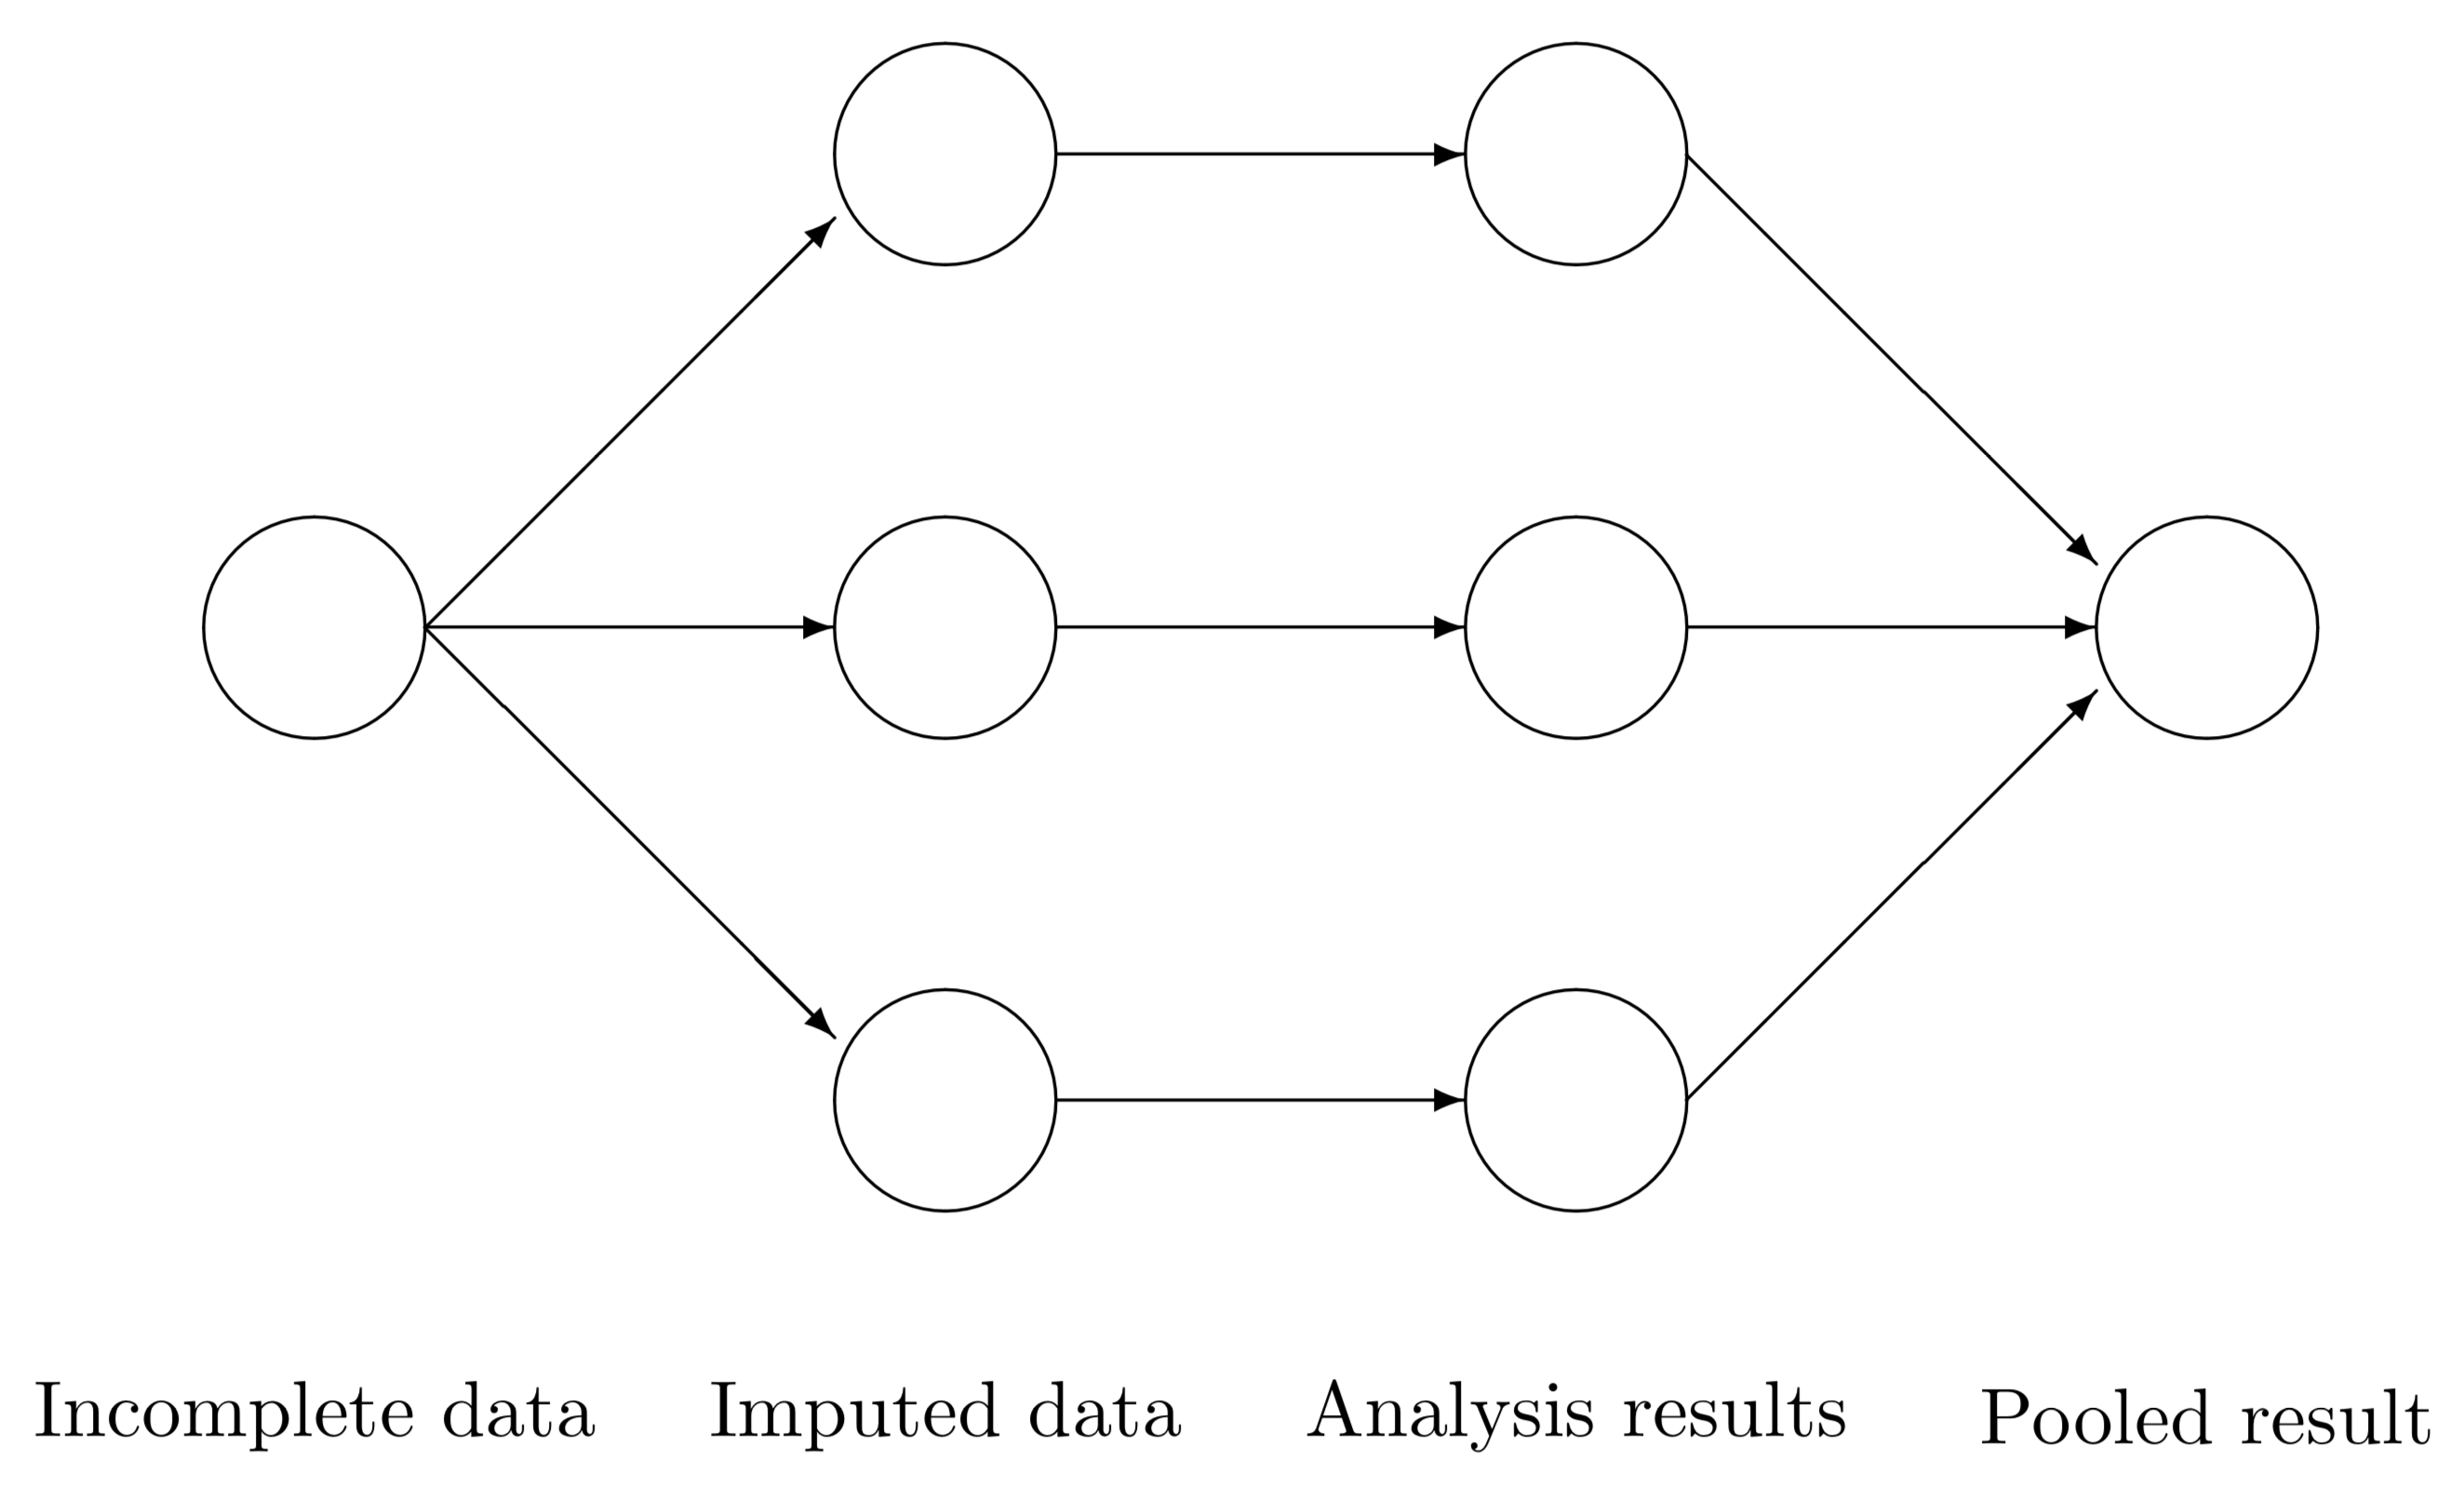
\includegraphics[height=6cm,keepaspectratio=true]{figures/ch01-miflow-1.png}}

\end{frame}

\begin{frame}{Acceptance of multiple imputation}
\protect\hypertarget{acceptance-of-multiple-imputation}{}

\begin{figure}
\includegraphics[height=2in]{Lecture_1_files/figure-beamer/unnamed-chunk-10-1} \caption{Source: Scopus (April 3, 2019)}\label{fig:unnamed-chunk-10}
\end{figure}

\end{frame}

\begin{frame}{Pooled estimate \(\bar Q\)}
\protect\hypertarget{pooled-estimate-bar-q}{}

\(\hat Q_\ell\) is the estimate of the \(\ell\)-th repeated imputation

\(\hat Q_\ell\) contains \(k\) parameters, represented as a
\(k \times 1\) column vector

Pooled estimate \(\bar Q\) is simply the average

\[ 
\bar Q = \frac{1}{m}\sum_{\ell=1}^m \hat Q_\ell
\]

\end{frame}

\begin{frame}{Within-imputation variance}
\protect\hypertarget{within-imputation-variance}{}

Average of the complete-data variances as

\[
  \bar U = \frac{1}{m}\sum_{\ell=1}^m \bar U_\ell,
\]

where \(\bar U_\ell\) is the variance-covariance matrix of
\(\hat Q_\ell\) obtained for the \(\ell\)-th imputation

\(\bar U_\ell\) is the variance is the estimate, \emph{not} the variance
in the data

Within-imputation variance is large if the sample is small

\end{frame}

\begin{frame}{Between-imputation variance}
\protect\hypertarget{between-imputation-variance}{}

Variance between the \(m\) complete-data estimates is given by

\[
B = \frac{1}{m-1}\sum_{\ell=1}^m (\hat Q_\ell-\bar Q)(\hat Q_\ell-\bar Q)',
\]

where \(\bar Q\) is the pooled estimate.

The between-imputation variance is large there many missing data

\end{frame}

\begin{frame}{Total variance}
\protect\hypertarget{total-variance}{}

The total variance is \emph{not} simply \(T=\bar U + B\)

The correct formula is

\begin{eqnarray}
  T & = & \bar U + B + B/m \nonumber \\
      & = & \bar U + \left(1+\frac{1}{m}\right)B
\end{eqnarray}

for the total variance of \(\bar Q_m\), and hence of \((Q-\bar Q)\) if
\(\bar Q\) is unbiased

The term \(B/m\) is the simulation error

\end{frame}

\begin{frame}{Three sources of variation}
\protect\hypertarget{three-sources-of-variation}{}

In summary, the total variance \(T\) stems from three sources:

\begin{enumerate}
\tightlist
\item
  \(\bar U\), the variance caused by the fact that we are taking a
  sample rather than the entire population. This is the conventional
  statistical measure of variability;
\item
  \(B\), the extra variance caused by the fact that there are missing
  values in the sample;
\item
  \(B/m\), the extra simulation variance caused by the fact that
  \(\bar Q_m\) itself is based on finite \(m\).
\end{enumerate}

\end{frame}

\begin{frame}{Variance ratio's (1)}
\protect\hypertarget{variance-ratios-1}{}

Proportion of the variation attributable to the missing data

\[
  \lambda = \frac{B+B/m}{T}
\]

Relative increase in variance due to nonresponse

\[
  r = \frac{B+B/m}{\bar U}
\]

These are related by \(r = \lambda/(1-\lambda)\).

\end{frame}

\begin{frame}{Variance ratio's (2)}
\protect\hypertarget{variance-ratios-2}{}

Fraction of information about \(Q\) missing due to nonresponse

\[
\gamma = \frac{r+2/(\nu+3)}{1+r}\label{eq:gammama}
\]

This measure needs an estimate of the degrees of freedom \(\nu\) (c.f.
section 2.3.6)

Relation between \(\gamma\) and \(\lambda\)

\[
\gamma = \frac{\nu+1}{\nu+3}\lambda+\frac{2}{\nu+3}.\label{eq:gammamb}
\]

The literature often confuses \(\gamma\) and \(\lambda\).

\end{frame}

\begin{frame}{Statistical inference for \(\bar Q\) (1)}
\protect\hypertarget{statistical-inference-for-bar-q-1}{}

The \(100(1-\alpha)\)\% confidence interval of a \(\bar Q\) is
calculated as

\[
\bar Q \pm t_{(\nu,1-\alpha/2)}\sqrt{T},
\]

where \(t_{(\nu,1-\alpha/2)}\) is the quantile corresponding to
probability \(1-\alpha/2\) of \(t_\nu\).

For example, use \(t(10,0.975)=2.23\) for the 95\% confidence interval
for \(\nu=10\).

\end{frame}

\begin{frame}{Statistical inference for \(\bar Q\) (2)}
\protect\hypertarget{statistical-inference-for-bar-q-2}{}

Suppose we test the null hypothesis \(Q=Q_0\) for some specified value
\(Q_0\). We can find the \(P\)-value of the test as the probability

\[
  P_s = \Pr\left[F_{1,\nu} > \frac{(Q_0 - \bar Q)^2}{T}\right]
\]

where \(F_{1,\nu}\) is an \(F\) distribution with 1 and \(\nu\) degrees
of freedom.

\end{frame}

\begin{frame}{How large should \(m\) be?}
\protect\hypertarget{how-large-should-m-be}{}

Classic advice: \(m=3, 5, 10\). More recently: set \(m\) higher:
20--100.

Some advice:

\begin{itemize}
\tightlist
\item
  Use \(m=5\) or \(m=10\) if the fraction of missing information is low,
  \(\gamma <0.2\).
\item
  Develop your model with \(m=5\). Do final run with \(m\) equal to
  percentage of incomplete cases.
\end{itemize}

\end{frame}

\begin{frame}{Multiple imputation in \texttt{mice}}
\protect\hypertarget{multiple-imputation-in-mice}{}

\centering{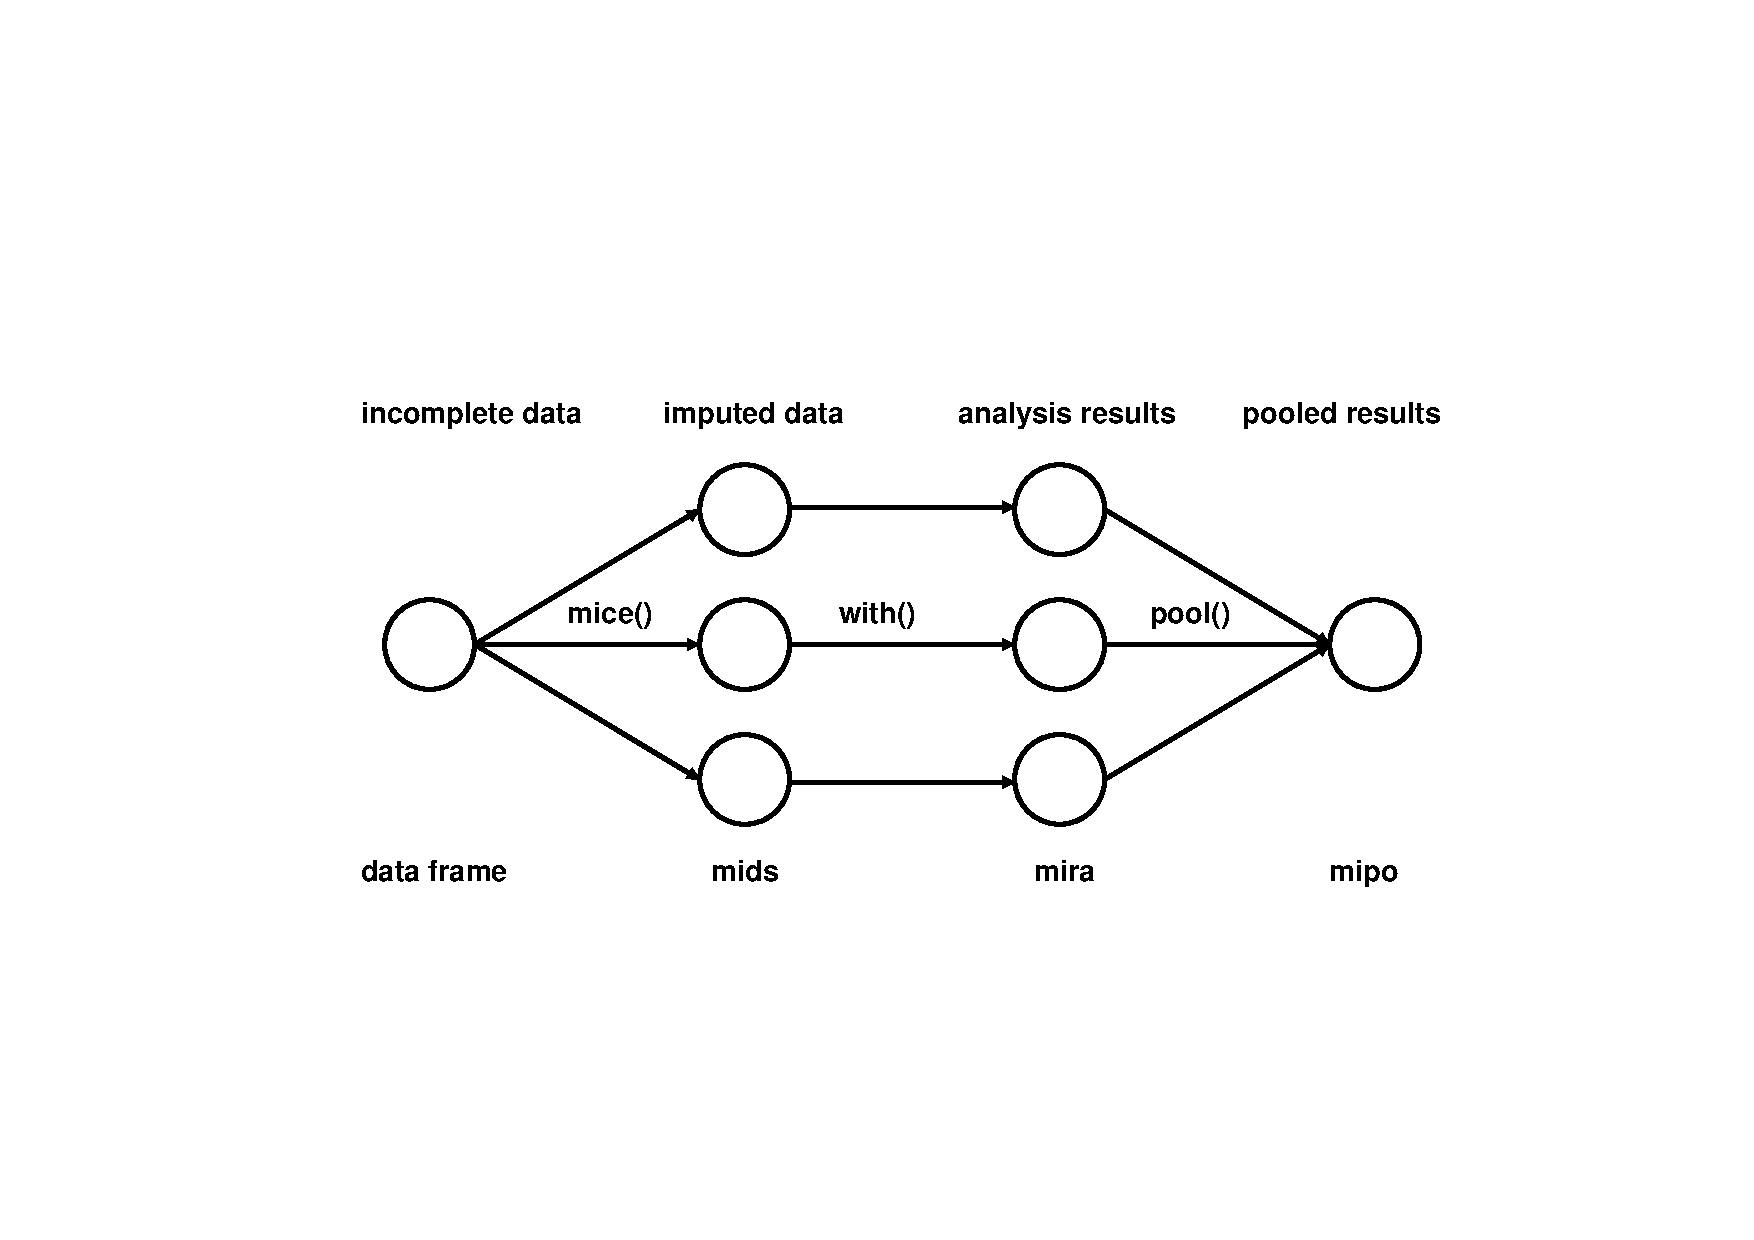
\includegraphics[height=8cm,keepaspectratio=true]{figures/figure1a.pdf}}

\end{frame}

\begin{frame}[fragile]{Inspect the data}
\protect\hypertarget{inspect-the-data}{}

\begin{Shaded}
\begin{Highlighting}[]
\KeywordTok{library}\NormalTok{(}\StringTok{"mice"}\NormalTok{)}
\KeywordTok{head}\NormalTok{(nhanes)}
\end{Highlighting}
\end{Shaded}

\begin{verbatim}
##   age  bmi hyp chl
## 1   1   NA  NA  NA
## 2   2 22.7   1 187
## 3   1   NA   1 187
## 4   3   NA  NA  NA
## 5   1 20.4   1 113
## 6   3   NA  NA 184
\end{verbatim}

\end{frame}

\begin{frame}[fragile]{Inspect missing data pattern}
\protect\hypertarget{inspect-missing-data-pattern}{}

\begin{Shaded}
\begin{Highlighting}[]
\KeywordTok{md.pattern}\NormalTok{(nhanes)}
\end{Highlighting}
\end{Shaded}

\begin{center}\includegraphics[height=3in]{Lecture_1_files/figure-beamer/unnamed-chunk-13-1} \end{center}

\begin{verbatim}
##    age hyp bmi chl   
## 13   1   1   1   1  0
## 3    1   1   1   0  1
## 1    1   1   0   1  1
## 1    1   0   0   1  2
## 7    1   0   0   0  3
##      0   8   9  10 27
\end{verbatim}

\end{frame}

\begin{frame}[fragile]{Multiply impute the data}
\protect\hypertarget{multiply-impute-the-data}{}

\begin{Shaded}
\begin{Highlighting}[]
\NormalTok{imp <-}\StringTok{ }\KeywordTok{mice}\NormalTok{(nhanes, }\DataTypeTok{print =} \OtherTok{FALSE}\NormalTok{, }\DataTypeTok{maxit=}\DecValTok{10}\NormalTok{, }\DataTypeTok{seed =} \DecValTok{24415}\NormalTok{)}
\end{Highlighting}
\end{Shaded}

\end{frame}

\begin{frame}{Inspect the trace lines for convergence}
\protect\hypertarget{inspect-the-trace-lines-for-convergence}{}

\includegraphics{Lecture_1_files/figure-beamer/unnamed-chunk-15-1.pdf}

\end{frame}

\begin{frame}[fragile]{Stripplot of observed and imputed data}
\protect\hypertarget{stripplot-of-observed-and-imputed-data}{}

\begin{Shaded}
\begin{Highlighting}[]
\KeywordTok{stripplot}\NormalTok{(imp, }\DataTypeTok{pch =} \DecValTok{20}\NormalTok{, }\DataTypeTok{cex =} \FloatTok{1.2}\NormalTok{)}
\end{Highlighting}
\end{Shaded}

\end{frame}

\begin{frame}{Stripplot of observed and imputed data}
\protect\hypertarget{stripplot-of-observed-and-imputed-data-1}{}

\includegraphics{Lecture_1_files/figure-beamer/unnamed-chunk-17-1.pdf}

\end{frame}

\begin{frame}[fragile]{Fit the complete-data model}
\protect\hypertarget{fit-the-complete-data-model}{}

\begin{Shaded}
\begin{Highlighting}[]
\NormalTok{fit <-}\StringTok{ }\KeywordTok{with}\NormalTok{(imp, }\KeywordTok{lm}\NormalTok{(bmi }\OperatorTok{~}\StringTok{ }\NormalTok{age))}
\NormalTok{est <-}\StringTok{ }\KeywordTok{pool}\NormalTok{(fit)}
\KeywordTok{summary}\NormalTok{(est)}
\end{Highlighting}
\end{Shaded}

\begin{verbatim}
##             estimate std.error statistic   df  p.value
## (Intercept)    30.69      2.09     14.70 13.4 1.16e-09
## age            -2.35      1.01     -2.33 17.4 3.23e-02
\end{verbatim}

\end{frame}

\begin{frame}{Temperature and gas consumption}
\protect\hypertarget{temperature-and-gas-consumption}{}

\includegraphics[height=3in]{Lecture_1_files/figure-beamer/gas2-1}

\end{frame}

\begin{frame}{Delete gas consumption of day 47}
\protect\hypertarget{delete-gas-consumption-of-day-47}{}

\includegraphics[height=3in]{Lecture_1_files/figure-beamer/unnamed-chunk-20-1}

\end{frame}

\begin{frame}{Predict value from regression line}
\protect\hypertarget{predict-value-from-regression-line}{}

\includegraphics[height=3in]{Lecture_1_files/figure-beamer/unnamed-chunk-21-1}

\end{frame}

\begin{frame}{Predict value + add noise}
\protect\hypertarget{predict-value-add-noise}{}

\includegraphics[height=3in]{Lecture_1_files/figure-beamer/unnamed-chunk-22-1}

\end{frame}

\begin{frame}{Predict + noise + parameter draw}
\protect\hypertarget{predict-noise-parameter-draw}{}

\includegraphics[height=3in]{Lecture_1_files/figure-beamer/unnamed-chunk-23-1}

\end{frame}

\begin{frame}{Two predictors}
\protect\hypertarget{two-predictors}{}

\includegraphics[height=3in]{Lecture_1_files/figure-beamer/unnamed-chunk-24-1}

\end{frame}

\begin{frame}{Drawing from observed data}
\protect\hypertarget{drawing-from-observed-data}{}

\includegraphics[height=3in]{Lecture_1_files/figure-beamer/unnamed-chunk-25-1}

\end{frame}

\begin{frame}{Multivariate missing data}
\protect\hypertarget{multivariate-missing-data}{}

\end{frame}

\begin{frame}{Missing data patterns}
\protect\hypertarget{missing-data-patterns}{}

\includegraphics{Lecture_1_files/figure-beamer/patterns-1.pdf}

\end{frame}

\begin{frame}{Three general strategies}
\protect\hypertarget{three-general-strategies}{}

\begin{itemize}
\tightlist
\item
  Monotone data imputation
\item
  Joint modeling
\item
  Fully conditional specification (FCS)
\end{itemize}

\end{frame}

\begin{frame}{Imputation of monotone pattern}
\protect\hypertarget{imputation-of-monotone-pattern}{}

\begin{center}\includegraphics[height=3in]{Lecture_1_files/figure-beamer/unnamed-chunk-26-1} \end{center}

\end{frame}

\begin{frame}{Imputation of monotone pattern}
\protect\hypertarget{imputation-of-monotone-pattern-1}{}

\begin{center}\includegraphics[height=3in]{Lecture_1_files/figure-beamer/unnamed-chunk-27-1} \end{center}

\end{frame}

\begin{frame}{Imputation of monotone pattern}
\protect\hypertarget{imputation-of-monotone-pattern-2}{}

\begin{center}\includegraphics[height=3in]{Lecture_1_files/figure-beamer/unnamed-chunk-28-1} \end{center}

\end{frame}

\begin{frame}{Imputation of monotone pattern}
\protect\hypertarget{imputation-of-monotone-pattern-3}{}

\begin{center}\includegraphics[height=3in]{Lecture_1_files/figure-beamer/unnamed-chunk-29-1} \end{center}

\end{frame}

\begin{frame}{Imputation by joint modelling}
\protect\hypertarget{imputation-by-joint-modelling}{}

\begin{center}\includegraphics[height=3in]{Lecture_1_files/figure-beamer/unnamed-chunk-30-1} \end{center}

\end{frame}

\begin{frame}{Imputation by joint modelling}
\protect\hypertarget{imputation-by-joint-modelling-1}{}

\begin{center}\includegraphics[height=3in]{Lecture_1_files/figure-beamer/unnamed-chunk-31-1} \end{center}

\end{frame}

\begin{frame}{Imputation by joint modelling}
\protect\hypertarget{imputation-by-joint-modelling-2}{}

\begin{center}\includegraphics[height=3in]{Lecture_1_files/figure-beamer/unnamed-chunk-32-1} \end{center}

\end{frame}

\begin{frame}{Imputation by joint modelling}
\protect\hypertarget{imputation-by-joint-modelling-3}{}

\begin{center}\includegraphics[height=3in]{Lecture_1_files/figure-beamer/unnamed-chunk-33-1} \end{center}

\end{frame}

\begin{frame}{Joint modelling - next iteration}
\protect\hypertarget{joint-modelling---next-iteration}{}

\begin{center}\includegraphics[height=3in]{Lecture_1_files/figure-beamer/unnamed-chunk-34-1} \end{center}

\end{frame}

\begin{frame}{Joint modelling - next iteration}
\protect\hypertarget{joint-modelling---next-iteration-1}{}

\begin{center}\includegraphics[height=3in]{Lecture_1_files/figure-beamer/unnamed-chunk-35-1} \end{center}

\end{frame}

\begin{frame}{Fully conditional specification}
\protect\hypertarget{fully-conditional-specification}{}

\begin{center}\includegraphics[height=3in]{Lecture_1_files/figure-beamer/unnamed-chunk-36-1} \end{center}

\end{frame}

\begin{frame}{Fully conditional specification}
\protect\hypertarget{fully-conditional-specification-1}{}

\begin{center}\includegraphics[height=3in]{Lecture_1_files/figure-beamer/unnamed-chunk-37-1} \end{center}

\end{frame}

\begin{frame}{Fully conditional specification}
\protect\hypertarget{fully-conditional-specification-2}{}

\begin{center}\includegraphics[height=3in]{Lecture_1_files/figure-beamer/unnamed-chunk-38-1} \end{center}

\end{frame}

\begin{frame}{Fully conditional specification}
\protect\hypertarget{fully-conditional-specification-3}{}

\begin{center}\includegraphics[height=3in]{Lecture_1_files/figure-beamer/unnamed-chunk-39-1} \end{center}

\end{frame}

\begin{frame}{Fully conditional specification}
\protect\hypertarget{fully-conditional-specification-4}{}

\begin{center}\includegraphics[height=3in]{Lecture_1_files/figure-beamer/unnamed-chunk-40-1} \end{center}

\end{frame}

\begin{frame}{Fully conditional specification - next}
\protect\hypertarget{fully-conditional-specification---next}{}

\begin{center}\includegraphics[height=3in]{Lecture_1_files/figure-beamer/unnamed-chunk-41-1} \end{center}

\end{frame}

\begin{frame}{Fully conditional specification - next}
\protect\hypertarget{fully-conditional-specification---next-1}{}

\begin{center}\includegraphics[height=3in]{Lecture_1_files/figure-beamer/unnamed-chunk-42-1} \end{center}

\end{frame}

\begin{frame}{How many iterations?}
\protect\hypertarget{how-many-iterations}{}

\begin{itemize}
\tightlist
\item
  Quick convergence
\item
  5--10 iterations is adequate for most problems
\item
  More iterations is \(\lambda\) is high
\item
  Inspect the generated imputations
\item
  Monitor convergence to detect anomalies
\end{itemize}

\end{frame}

\begin{frame}{Non-convergence}
\protect\hypertarget{non-convergence}{}

\centering{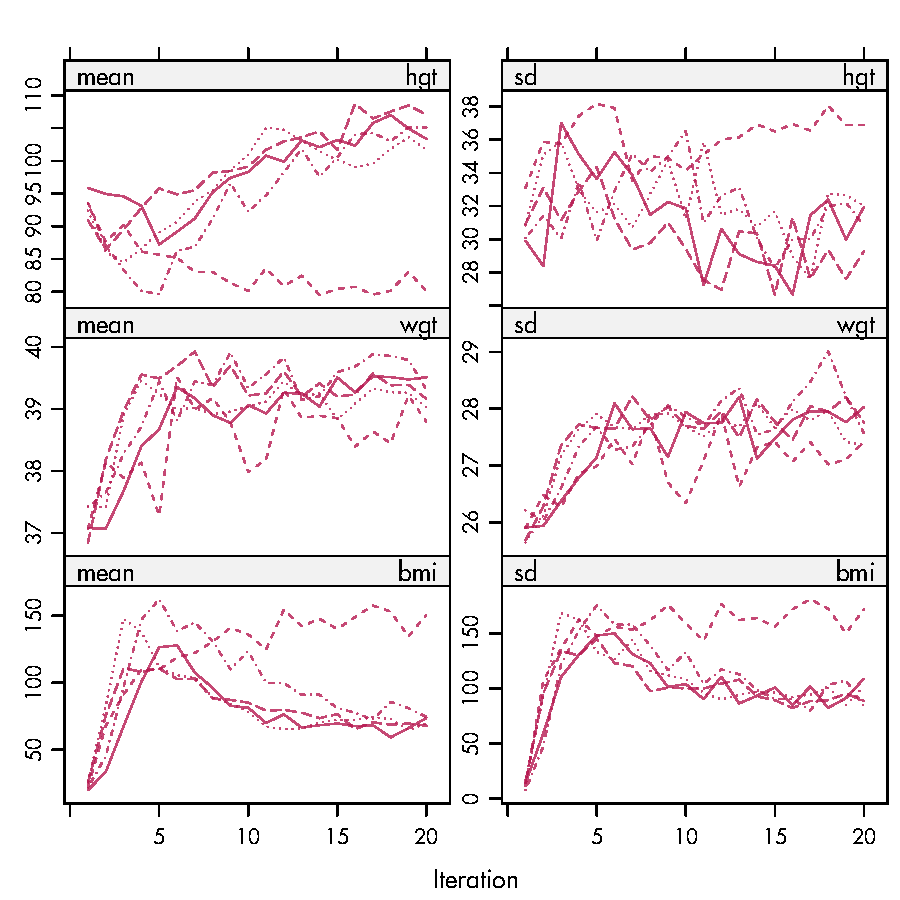
\includegraphics[height=8cm,keepaspectratio=true]{figures/ch5-convergence3}}

\end{frame}

\begin{frame}{Convergence}
\protect\hypertarget{convergence}{}

\centering{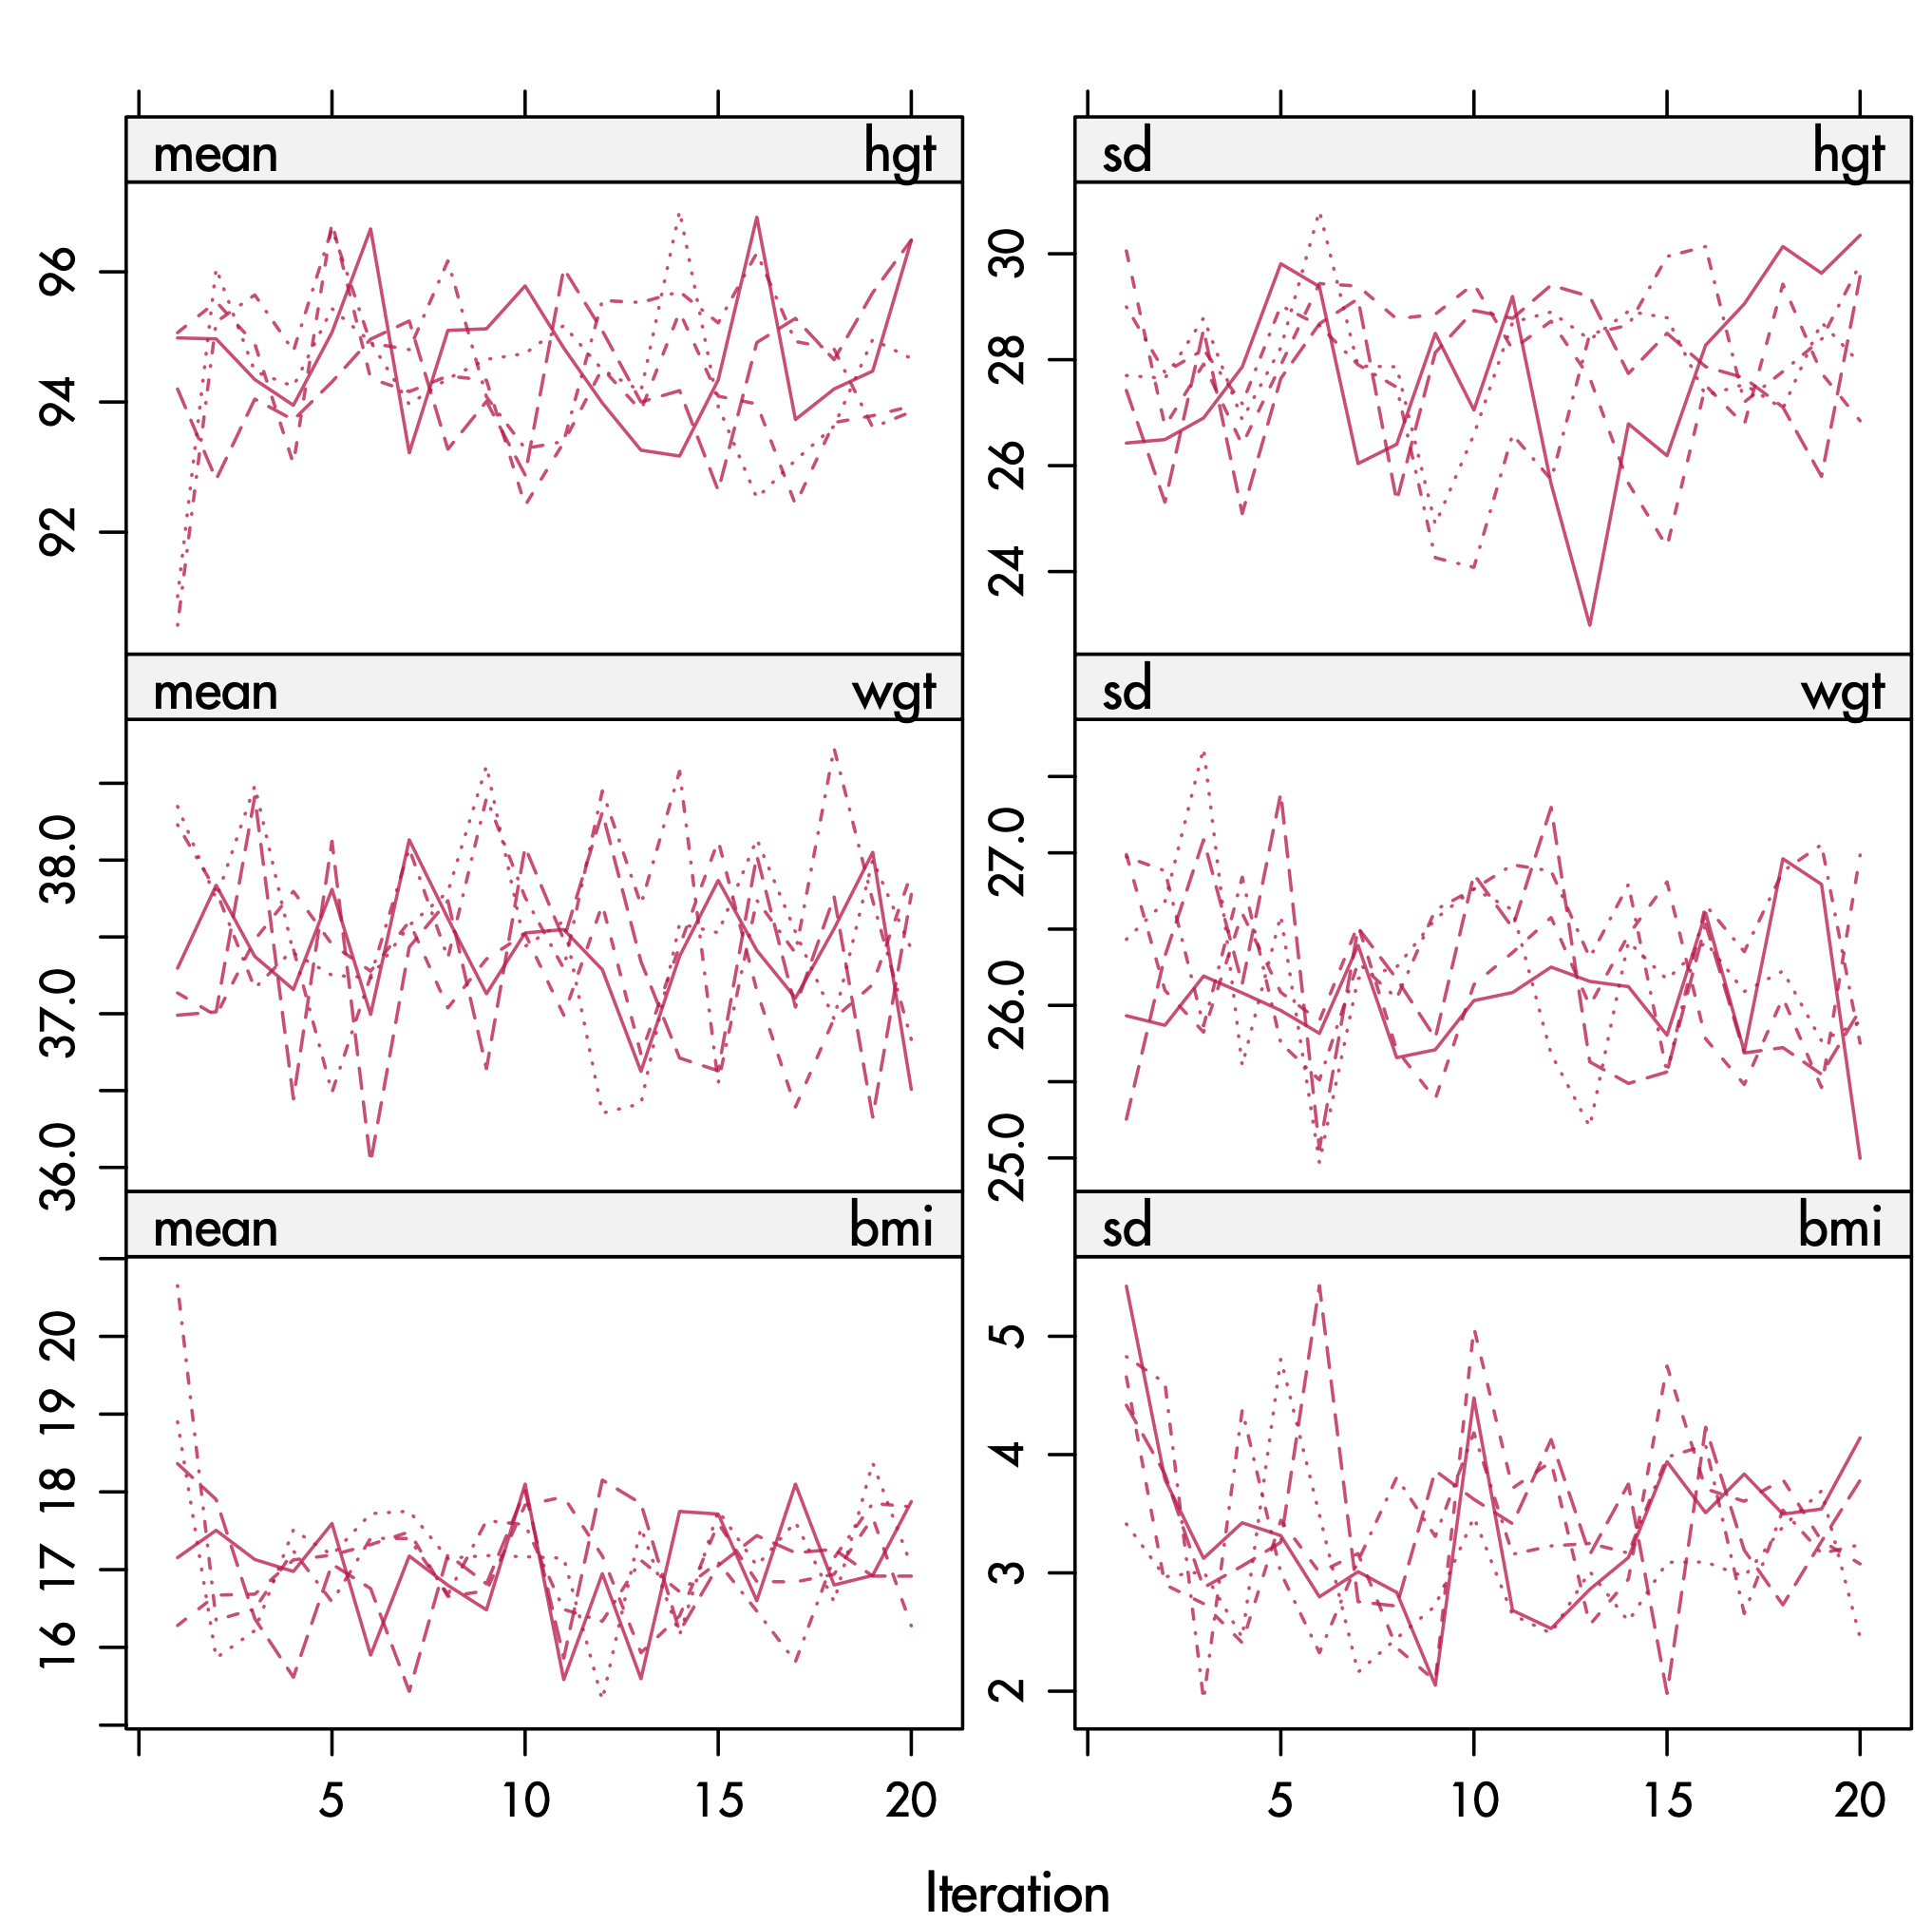
\includegraphics[height=8cm,keepaspectratio=true]{figures/ch5-convergence5}}

\end{frame}

\begin{frame}[fragile]{Conclusion}
\protect\hypertarget{conclusion}{}

\begin{itemize}
\tightlist
\item
  A general problem, a general solution
\item
  \texttt{mice} package: \textgreater{}50,000 downloads per month
\item
  Highly useful for data combination
\end{itemize}

\end{frame}

\end{document}
